\documentclass{beamer}
\usepackage[english, russian]{babel}
\usepackage[T2A]{fontenc}
\usepackage[utf8]{inputenc}
\usepackage{indentfirst}
\usepackage{amsmath, amsfonts, amssymb, amsthm, mathtools}
\usepackage[export]{adjustbox}
\usepackage{graphicx} 
\graphicspath{ {./images/} }

\usepackage{subcaption}
\usepackage{verbatim}

\usepackage{minted}{\setlength{\parskip}{0pt}}

\usepackage{hyperref}

\hypersetup{
    colorlinks=true,
    linkcolor=blue,
    filecolor=magenta,      
    urlcolor=black,
    pdftitle={Overleaf Example},
    pdfpagemode=FullScreen,
    }


\title{Лабораторная работа № 1. \\ Подготовка лабораторного стенда.}
\author{Данила Стариков \\ НПИбд-02-22}
\institute{Российский университет дружбы народов имени Патриса Лумумбы}
\date{2024}

\begin{document}

\frame{\titlepage}

\begin{frame}
\frametitle{Цель работы}
\begin{itemize}
    \item Приобретение практических навыков установки Rocky Linux на виртуальную машину с помощью инструмента Vagrant.
\end{itemize}
\end{frame}

\begin{frame}
\frametitle{Утилиты для работы}
\begin{itemize}
    \item Vagrant v2.3.4 (\url{https://vagrantup.com});
    \item VirtualBox v7.0.16 (\url{https://www.virtualbox.org}).
    \item Packer v1.11.2 (\url{https://www.packer.io}).
\end{itemize}
\end{frame}

\begin{frame}
\frametitle{Подготовка лабораторного стенда}
        \centering
    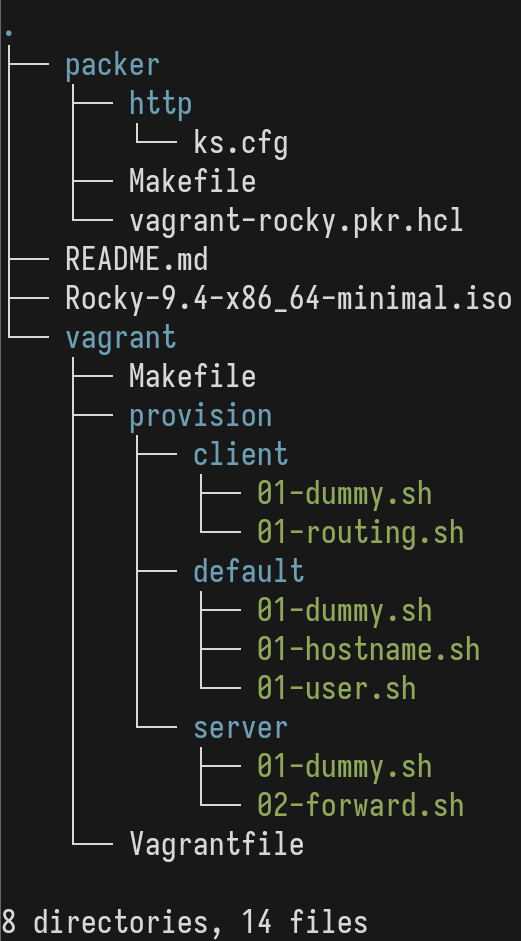
\includegraphics[height=0.8\textheight]{../images/img1.png}
    \captionof{figure}{Структура рабочего каталога.}
\end{frame}

\begin{frame}
\frametitle{Подготовка лабораторного стенда}
        \centering
    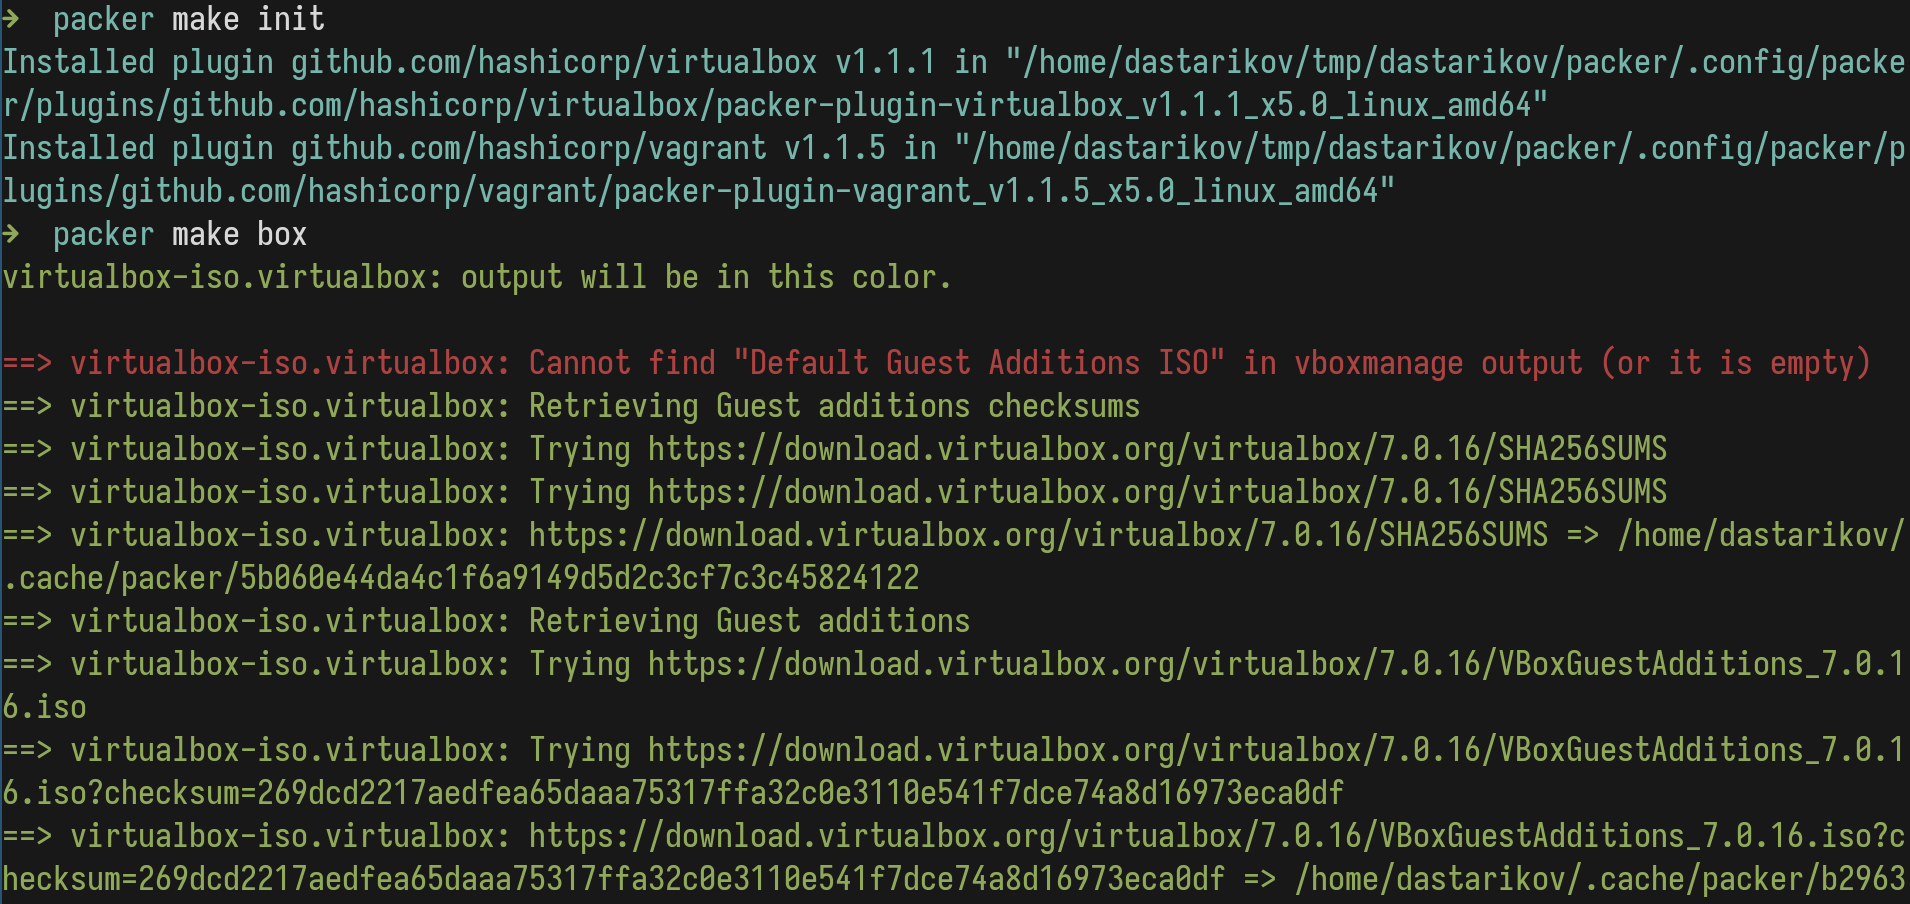
\includegraphics[width=\textwidth]{../images/img2.png}
    \captionof{figure}{Запуск формирования \texttt{box}-файла.}
\end{frame}

\begin{frame}
\frametitle{Подготовка лабораторного стенда}
        \centering
        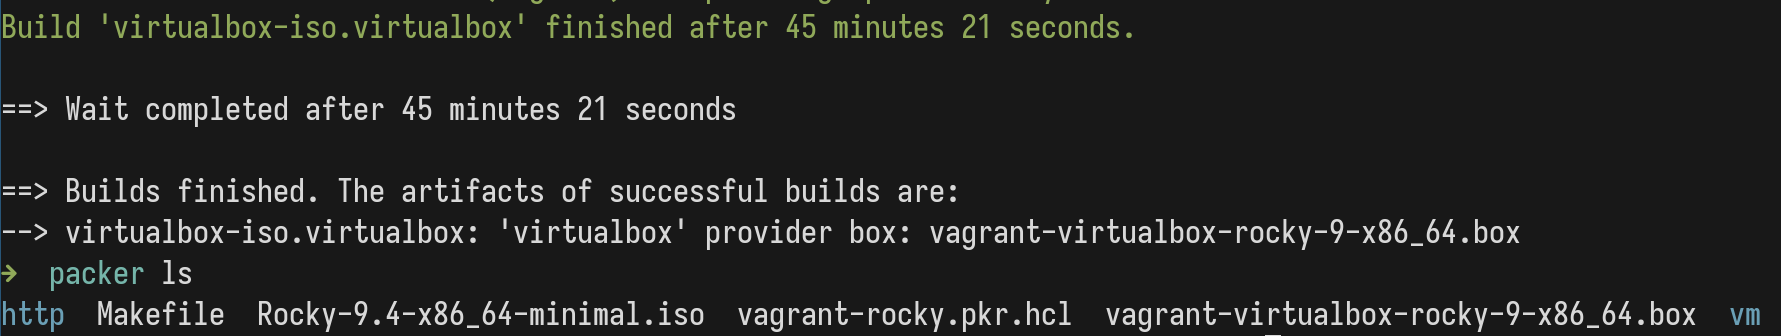
\includegraphics[width=\textwidth]{../images/img3.png}
        \captionof{figure}{Окончание сброки образа.}
        \centering
        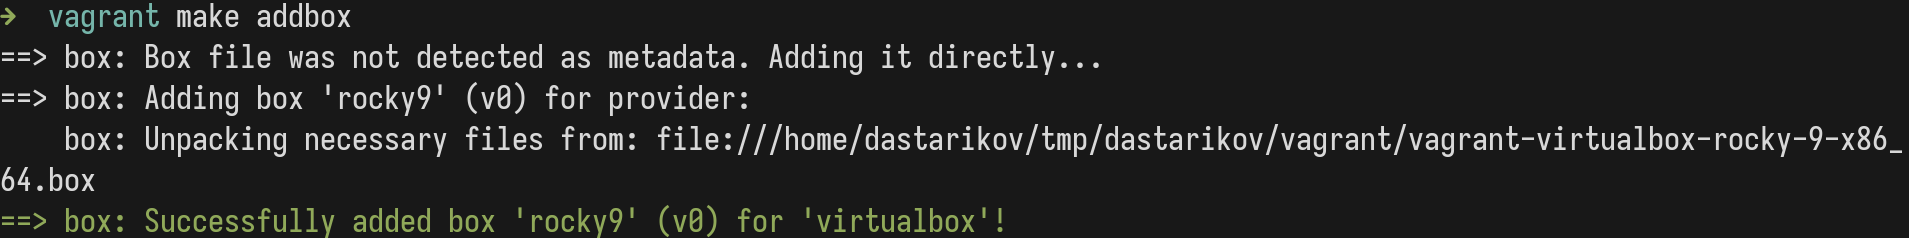
\includegraphics[width=\textwidth]{../images/img4.png}
        \captionof{figure}{Регистрация образа в Vagrant.}
\end{frame}

% \begin{frame}
% \frametitle{Подготовка лабораторного стенда}
% \end{frame}

\begin{frame}
\frametitle{Подготовка лабораторного стенда}
        \centering
        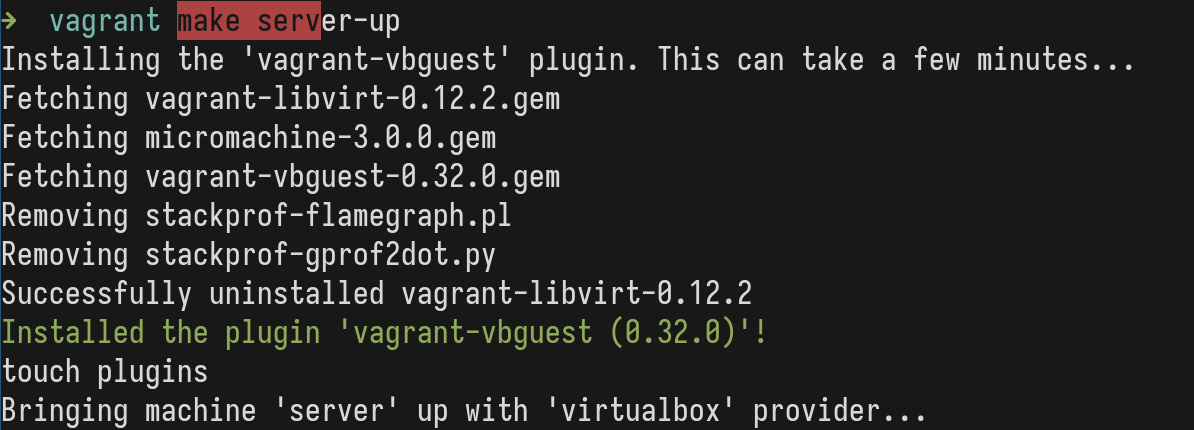
\includegraphics[width=\textwidth]{../images/img5.png}
        \captionof{figure}{Запуск виртуальной машины server}
\end{frame}
\begin{frame}
\frametitle{Подготовка лабораторного стенда}
        \centering
        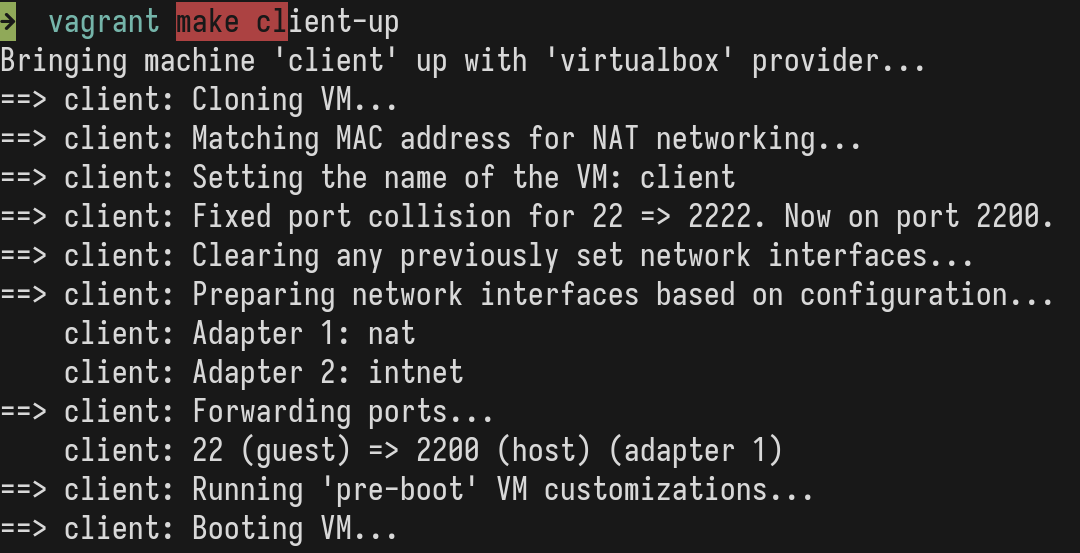
\includegraphics[width=\textwidth]{../images/img6.png}
        \captionof{figure}{Запуск виртуальной машины client}
\end{frame}
\begin{frame}
\frametitle{Подключение по ssh}
        \centering
        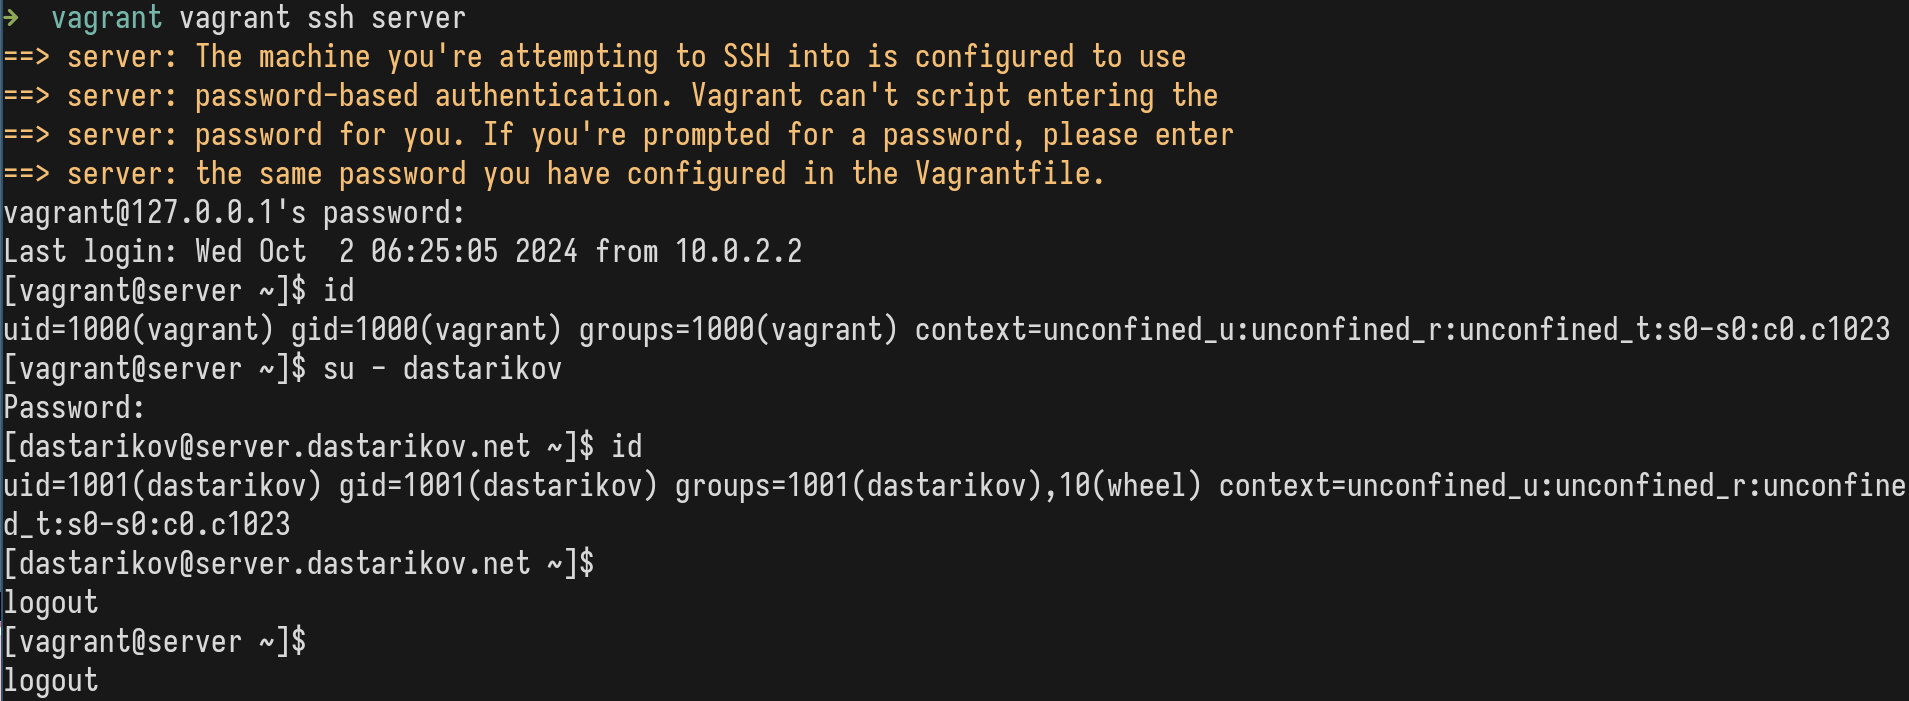
\includegraphics[width=0.8\textwidth]{../images/img7.png}
        \captionof{figure}{Подключение к серверу из консоли.}
        \centering
        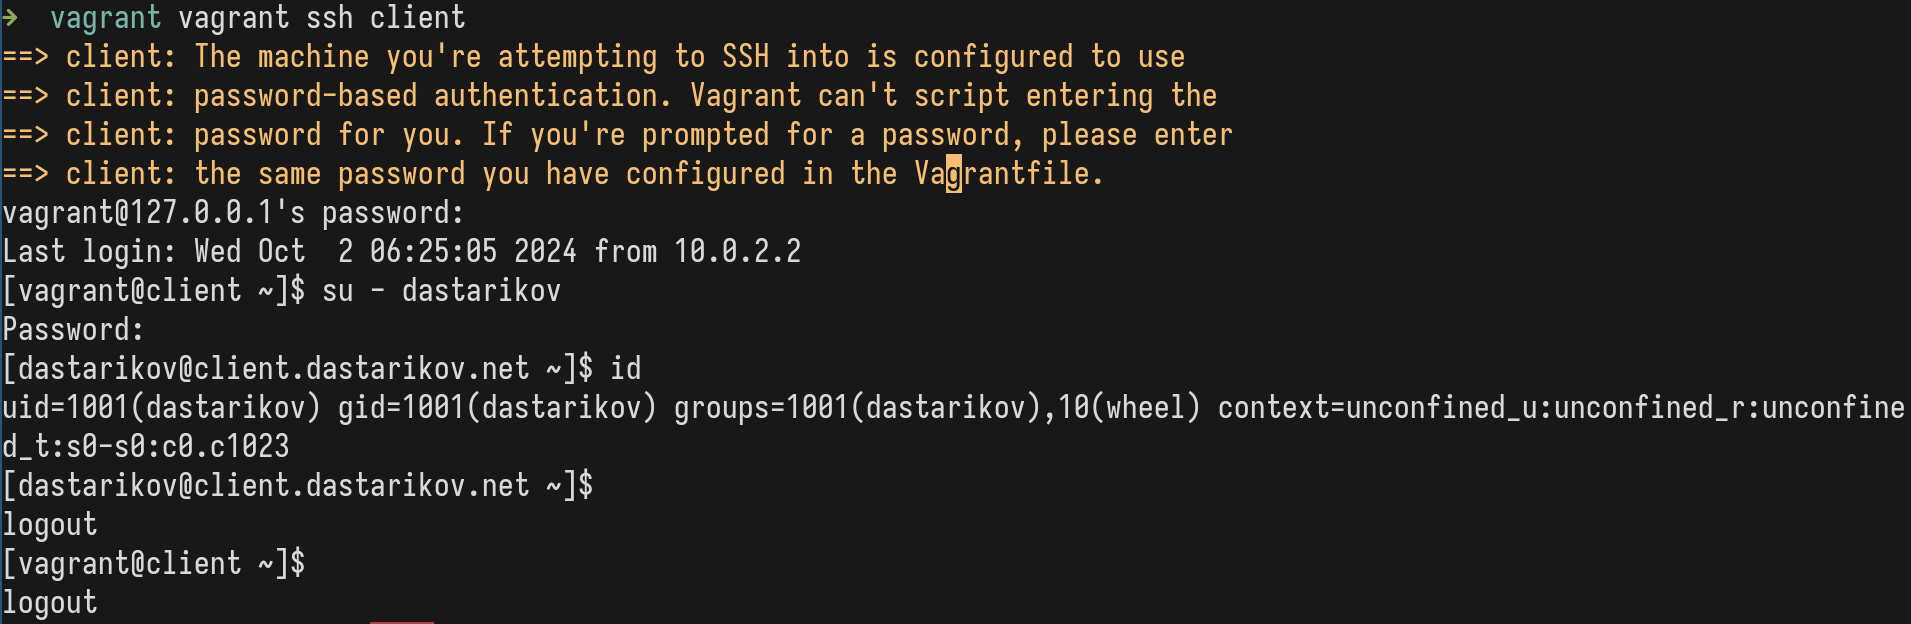
\includegraphics[width=0.8\textwidth]{../images/img7a.png}
        \captionof{figure}{Подключение к клиенту из консоли.}
% \begin{columns}
%     \column{0.5\textwidth}
%     \column{0.5\textwidth}
% \end{columns}
\end{frame}

\begin{frame}
\frametitle{Подготовка лабораторного стенда}
        \centering
        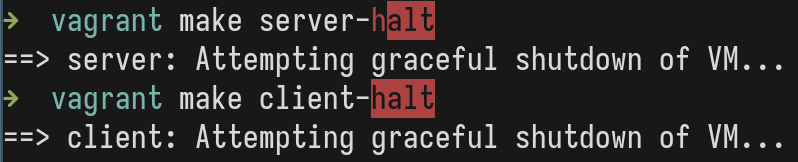
\includegraphics[width=\textwidth]{../images/img8.png}

        \captionof{figure}{Выключение виртуальных машин.}
\end{frame}

\begin{frame}
\frametitle{Подготовка лабораторного стенда}
\begin{columns}
    \column{0.5\textwidth}
        \centering
        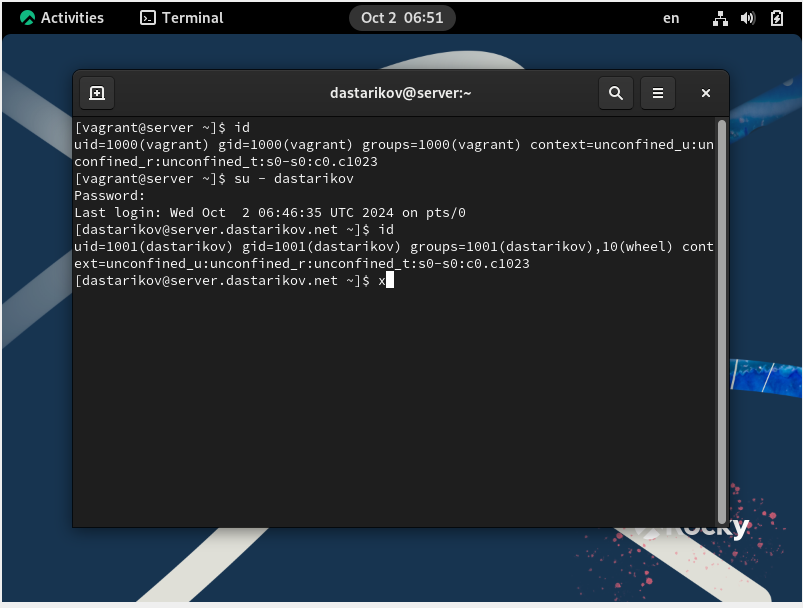
\includegraphics[width=\textwidth]{../images/img9.png}
        \captionof{figure}{Работа в графическом окружении сервера.}
    \column{0.5\textwidth}
        \centering
        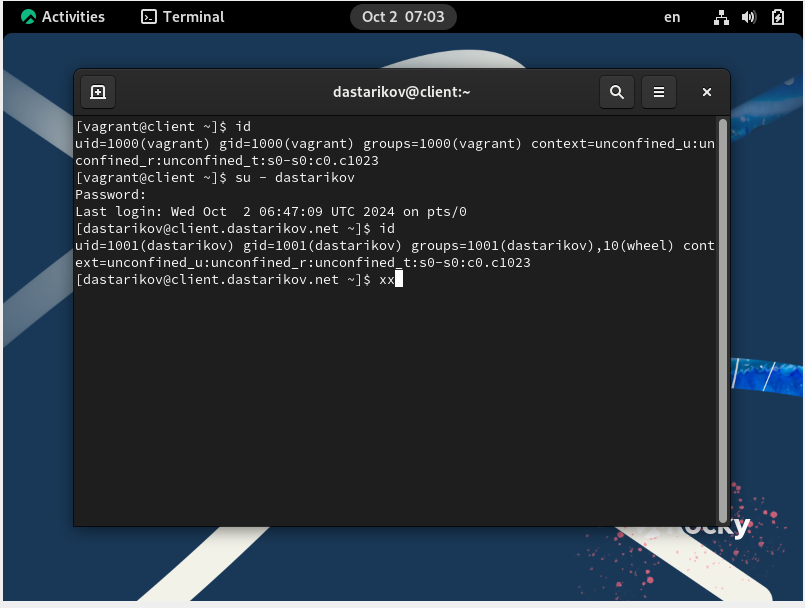
\includegraphics[width=\textwidth]{../images/img10.png}
        \captionof{figure}{Работа в графическом окружении клиента.}
\end{columns}
\end{frame}

\begin{frame}[containsverbatim]
\frametitle{Внесение изменений в настройки внутреннего окружения}
        \begin{minted}{bash}
        # Common configuration
        config.vm.provision "common user",
        type: "shell",
        preserve_order: true,
        path: "provision/default/01-user.sh"
        config.vm.provision "common hostname",
        type: "shell",
        preserve_order: true,
        run: "always",
        path: "provision/default/01-hostname.sh"
        \end{minted}
\end{frame}

\begin{frame}
\frametitle{Внесение изменений в настройки внутреннего окружения}
\begin{columns}
    \column{0.5\textwidth}
        \centering
        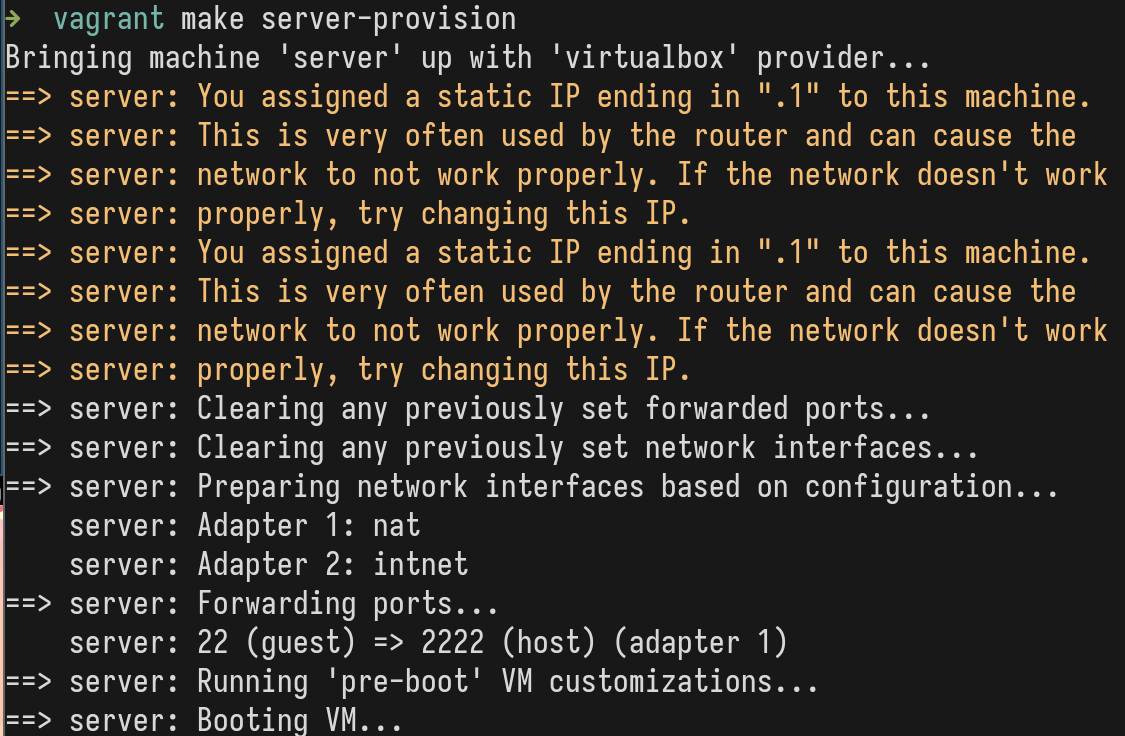
\includegraphics[width=\textwidth]{../images/img11.png}
        \captionof{figure}{Фиксирование изменений настроек сервера.}
    \column{0.5\textwidth}
        \centering
        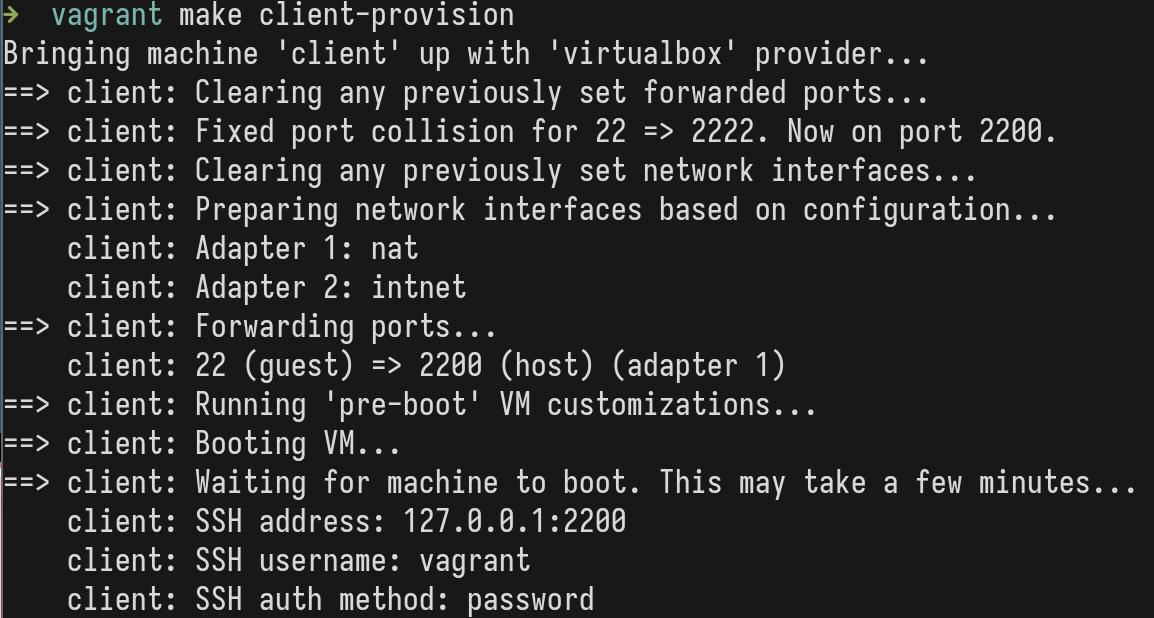
\includegraphics[width=\textwidth]{../images/img12.png}
        \captionof{figure}{Фиксирование изменений настроек клиента.}
\end{columns}
\end{frame}


\begin{frame}
\frametitle{Внесение изменений в настройки внутреннего окружения}
\begin{columns}
    \column{0.5\textwidth}
        \centering
        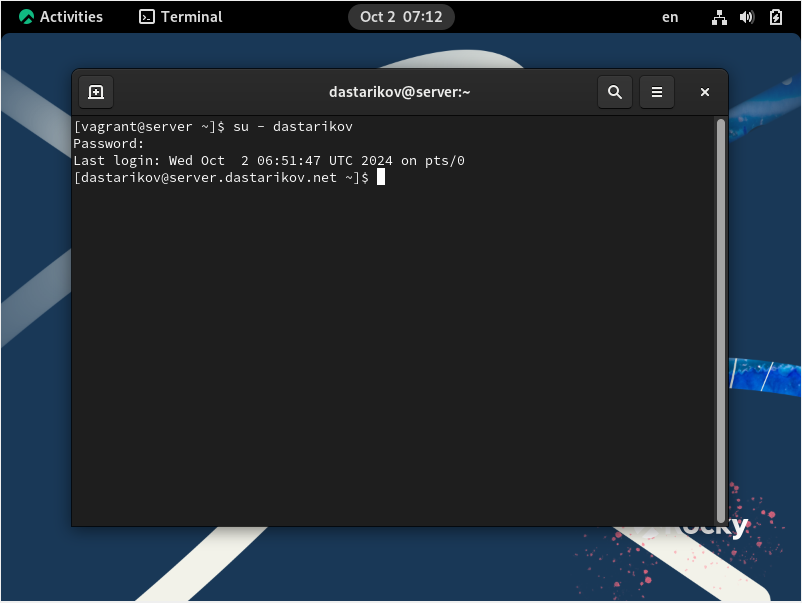
\includegraphics[width=\textwidth]{../images/img13.png}
        \captionof{figure}{Проверка отображения приглашения на сервере.}
    \column{0.5\textwidth}
        \centering
        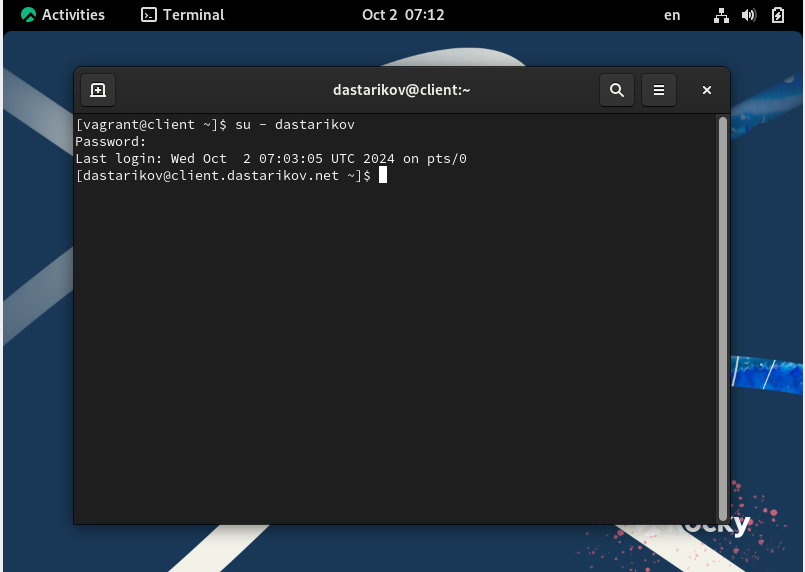
\includegraphics[width=\textwidth]{../images/img14.png}
        \captionof{figure}{Проверка отображения приглашения на клиенте.}
\end{columns}
\end{frame}

\begin{frame}
\frametitle{Выводы}
\begin{itemize}
    \item В рамках лабораторной работы познакомились с инструментом Vagrant и подготовили лабораторный стенд.
\end{itemize}
\end{frame}
\end{document}
